\documentclass[presentation]{beamer}

\usepackage{tikz}
\usetikzlibrary{positioning,calc,matrix}
\usetikzlibrary{shapes.geometric}
\usetikzlibrary{backgrounds}% only to show the bounding box
\usepackage{pgf}
\usepackage{pgfplots}
\usepackage{pgfplotstable}
\usepackage{appendixnumberbeamer}
\usepackage{amsmath}
\DeclareMathOperator{\tr}{tr}
\date{6th July 2017}
\usetheme{metropolis}
\metroset{progressbar=frametitle}

\renewcommand{\vec}[1]{\ensuremath{\boldsymbol{#1}}}
\newcommand{\ddt}[1]{\frac{\partial #1}{\partial t}}
\newcommand{\zhat}{\hat{\vec{z}}}
\newcommand{\W}{\ensuremath{\mathbb{W}}}

\newcommand{\inner}[1]{\left\langle #1 \right \rangle}

\newcommand{\KSP}[2]{\ensuremath{\mathcal{K}\left(#1, \mathbb{#2}\right)}}
\newcommand{\ksp}[1]{\KSP{#1}{#1}}

\newcommand{\highlight}[1]{\colorbox{red!20}{\color{black} #1}}
\newcommand{\arxivlink}[2]{%
  \href{http://www.arxiv.org/abs/#1}%
  {\texttt{arXiv:\,#1\,[#2]}}%
}
\newcommand{\doilink}[1]{%
  \href{http://dx.doi.org/#1}%
  {\texttt{doi:\,#1}{}}%
}

\author{Lawrence Mitchell\inst{1,*}}
\institute{
\inst{1}Departments of Computing and Mathematics, Imperial College
London

\inst{*}\texttt{lawrence.mitchell@imperial.ac.uk}
}

\graphicspath{{./\jobname.figures/}}

\usepackage[url=false,
            doi=true,
            isbn=false,
            style=authoryear,
            firstinits=true,
            uniquename=init,
            backend=biber]{biblatex}

\setbeamertemplate{bibliography item}{}

\renewcommand{\bibfont}{\footnotesize}
\addbibresource{references.bib}

\setlength{\bibitemsep}{1ex}
\setlength{\fboxsep}{1pt}

\renewbibmacro{in:}{}
\DeclareFieldFormat[article]{volume}{\textbf{#1}}
\DeclareFieldFormat{doi}{%
  doi\addcolon%
  {\scriptsize\ifhyperref{\href{http://dx.doi.org/#1}{\nolinkurl{#1}}}
    {\nolinkurl{#1}}}}
\AtEveryBibitem{%
\clearfield{pages}%
\clearfield{issue}%
\clearfield{number}%
}

\usepackage{minted}
\RecustomVerbatimEnvironment{Verbatim}{BVerbatim}{}

\title{Symbolic numerical computing}
\begin{document}
\maketitle

\begin{frame}[t]
  \frametitle{A problem}
  \begin{itemize}
  \item Computational simulation of partial differential equations
    underpins much of modern science and engineering.
  \item Simulation models are ever more complex.
  \item The extra computational effort used to be offset by increased
    hardware performance \ldots
  \end{itemize}
  \begin{columns}
    \begin{column}{0.95\paperwidth}
      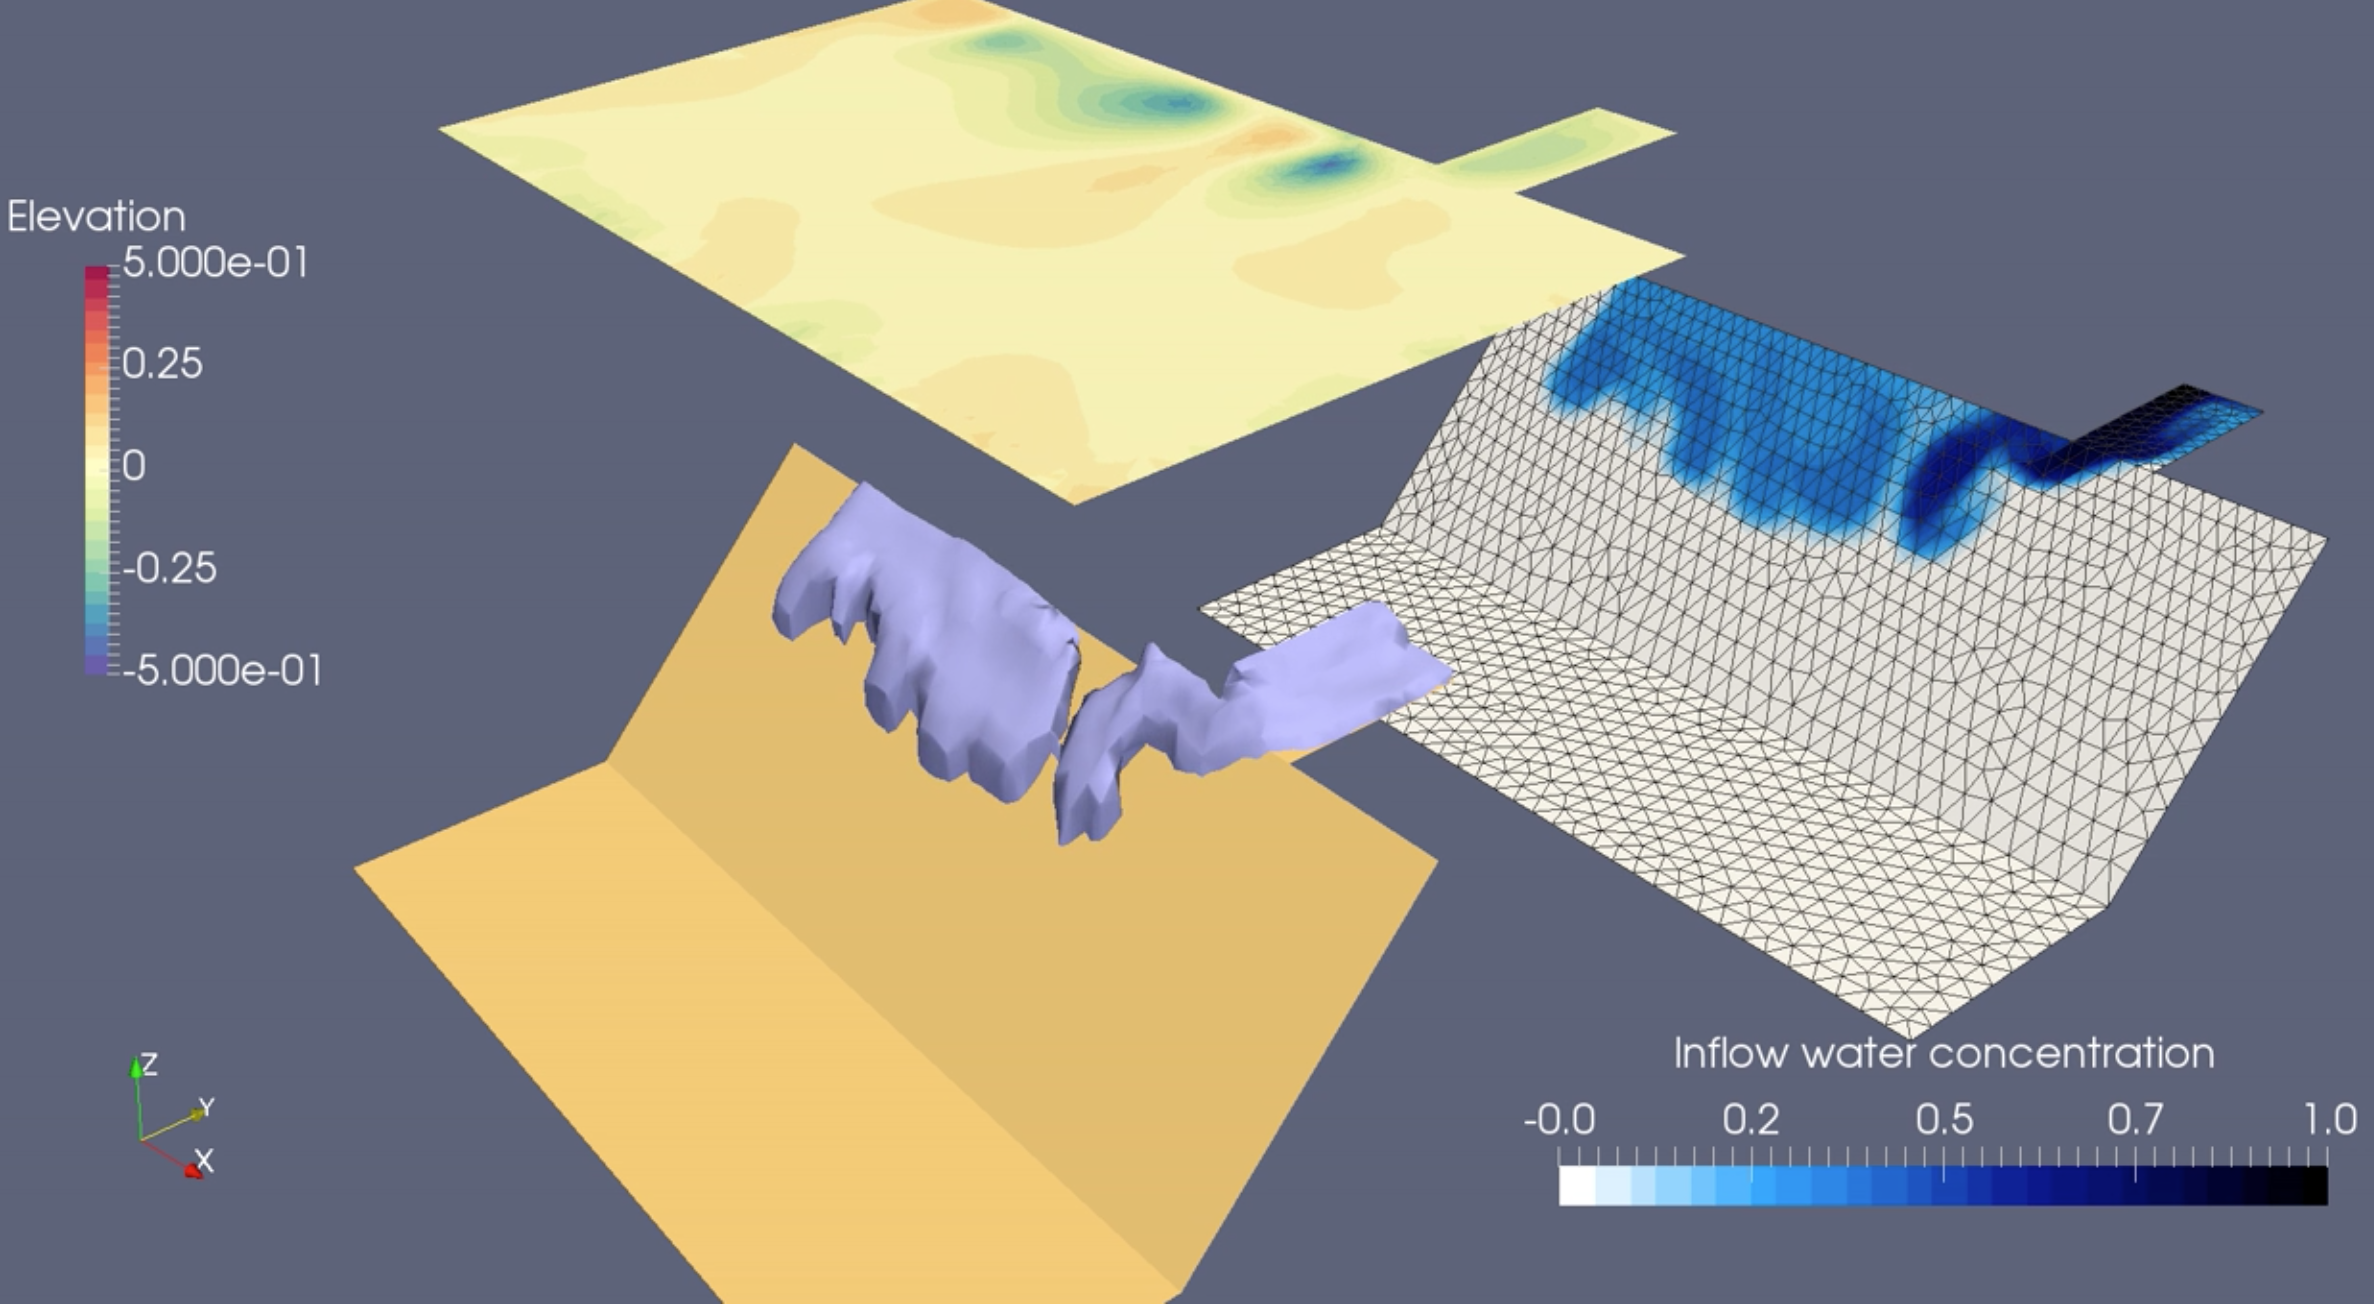
\includegraphics[height=4cm]{dome-entrainment}\hfill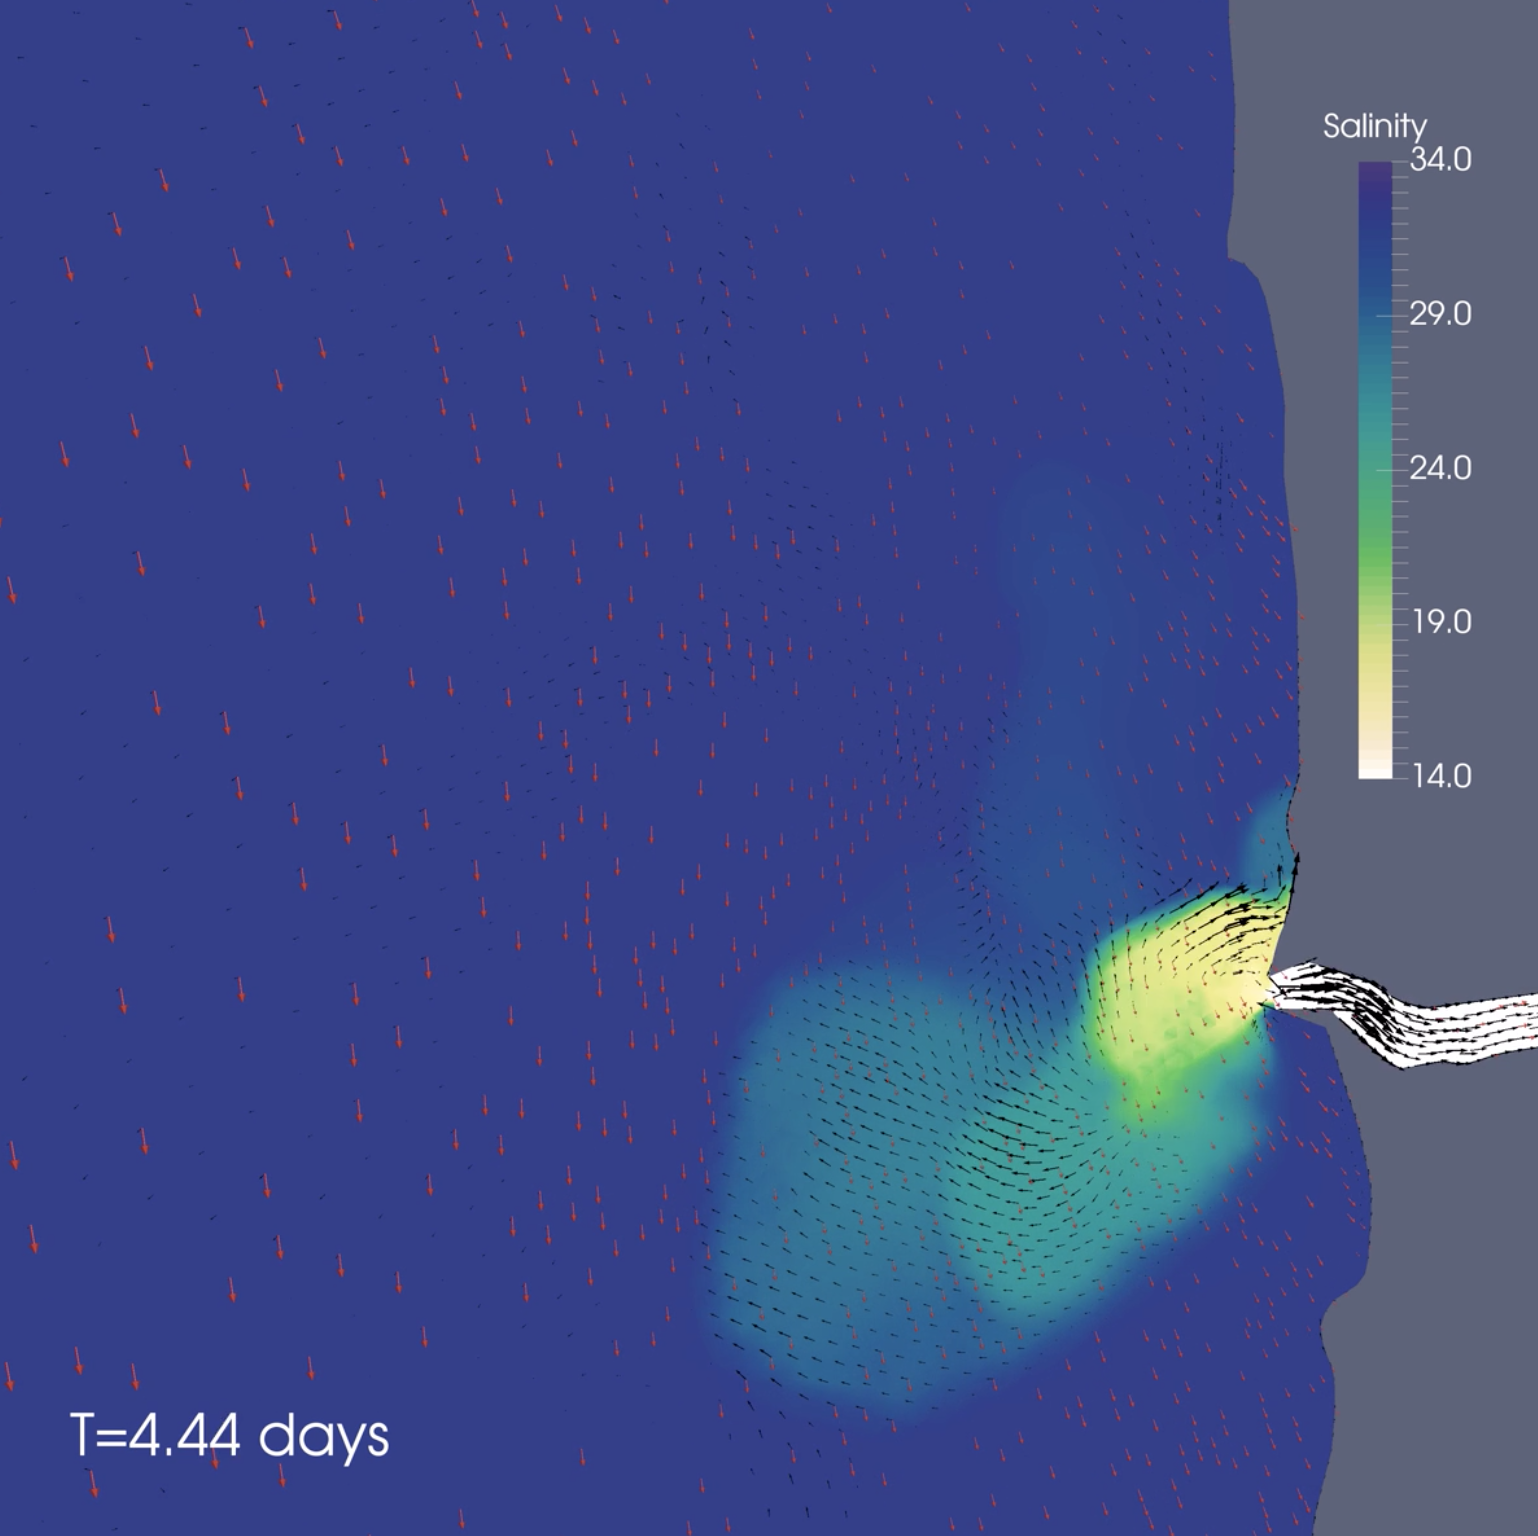
\includegraphics[height=4cm]{columbia-plume}
    \end{column}
  \end{columns}
\end{frame}

\begin{frame}
  \frametitle{The free lunch finished a long time ago}
    \begin{center}
      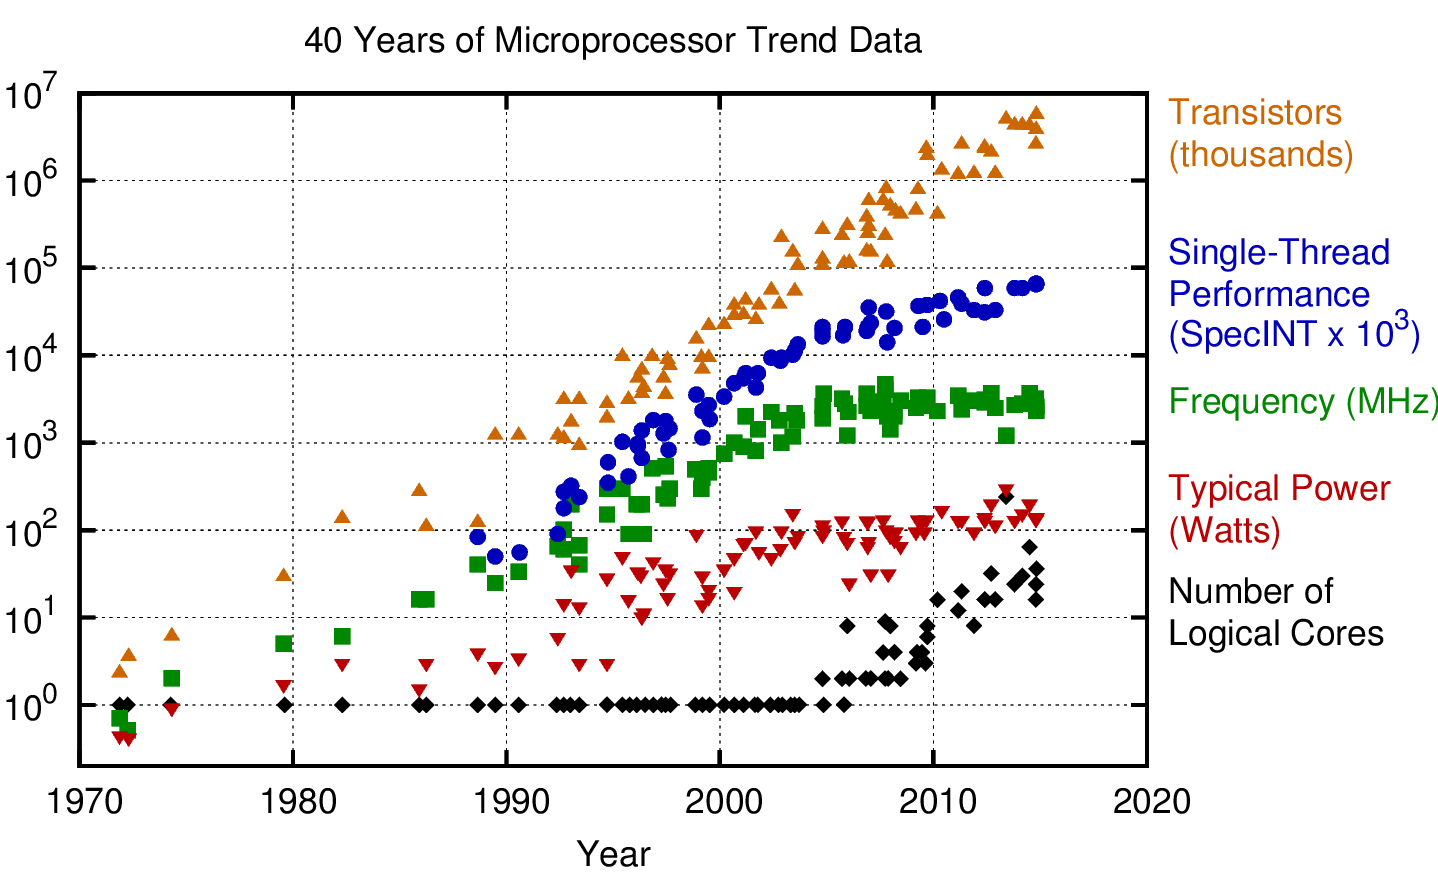
\includegraphics[height=0.5\textheight]{processor-trends}
    \end{center}
    \begin{flushright}
      {\tiny Figure courtesy Karl Rupp (CC-BY 4.0) \url{https://www.karlrupp.net/2015/06/40-years-of-microprocessor-trend-data/}}
    \end{flushright}
  \begin{itemize}
  \item Today's simulation models will run probably \emph{slower}, not faster, on
    tomorrow's hardware.
  \end{itemize}
\end{frame}

\begin{frame}
  \frametitle{What are the challenges?}
  \begin{itemize}
  \item Simulation software needs to exploit \emph{fine-grained}
    parallelism.
  \item Most code intimately intertwines the numerical algorithm with
    its \emph{implementation}.
  \item To apply program transformations, we have to unpick,
    understand, and reimplement.
  \end{itemize}
\end{frame}

\begin{frame}[fragile]
  \frametitle{Exploiting mathematical abstractions}
  Compute $y \leftarrow \nabla^2 x$ using finite differences.
  \begin{equation*}
    y_{i,j} = x_{i-1, j} + x_{i+1, j} + x_{i, j-1} + x_{i, j+1} - 4x_{i,j}    
  \end{equation*}
  \begin{overlayarea}{\textwidth}{0.8\textheight}
  \begin{onlyenv}<1>
    \begin{block}{Before 1953}
\begin{minted}[fontsize=\tiny]{asm}
        ...
        faddp   %st, %st(1)
        movl    -8(%ebp), %edx
        movl    %edx, %eax
        sall    $2, %eax
        addl    %edx, %eax
        leal    0(,%eax,4), %edx
        addl    %edx, %eax
        sall    $2, %eax
        movl    %eax, %edx
        movl    -4(%ebp), %eax
        addl    %edx, %eax
        subl    $101, %eax
        flds    x.3305(,%eax,4)
        flds    .LC0
        fmulp   %st, %st(1)
        faddp   %st, %st(1)
        fstps   y.3307(,%ecx,4)
        ...
\end{minted}
    \end{block}
  \end{onlyenv}
  \begin{onlyenv}<2->
    \begin{block}{After 1953}
\begin{minted}[fontsize=\tiny]{fortran}
      PROGRAM MAIN
      PARAMETER (N=100)
      REAL X(N,N), Y(N,N)
      DO 10 J=2,N-1
         DO 20 I=2,N-1
            Y(I,J)=X(I-1,J)+X(I+1,J)+X(I,J-1)+X(I,J+1)+4*X(I,J)
 20      CONTINUE
 10   CONTINUE
      DO 30 I=1,N
         Y(I,1) = 0.0
         Y(I,N) = 0.0
         Y(1,I) = 0.0
         Y(N,I) = 0.0
 30   CONTINUE
      END
\end{minted}
    \end{block}
  \end{onlyenv}
  \end{overlayarea}
\end{frame}

\begin{frame}
  \frametitle{Abstractions for PDE solvers}
  \begin{itemize}
  \item For complex numerical models, Fortran alone is not sufficient.
  \item One answer is software libraries.
  \item But these still put much of the burden on the model developer
  \item and transformations that cross library boundaries are hard.
  \item Instead, we use a domain specific language for specifying PDE
    solvers
  \item by saying \emph{what}, not \emph{how}, we can synthesise
    efficient implementations.
  \end{itemize}
\end{frame}

\begin{frame}
  \frametitle{Finite element crash course}
  \begin{align*}
    F(u) &= 0 \text{ in $\Omega$}\\
    u &= g \text{ on $\Gamma_1$}\\
    \frac{\partial u}{\partial n} &= h \text{ on $\Gamma_2$}
  \end{align*}
  Seek \emph{weak} solution in some space of functions $V(\Omega)$.

  Now we need to solve the (infinite dimensional) problem, find $u\in V$ s.t.
  \begin{equation*}
    \int_\Omega \!F(u) v\, \text{d}x = 0 \quad \forall\, v \in V
  \end{equation*}
\end{frame}
\begin{frame}
  \frametitle{Finite element crash course}
  Choose finite dimensional $V_h \subset V$, and seek a solution in
  that subspace: find $u_h \in V_h$ s.t.
  \begin{equation*}
    \int_\Omega \!F(u_h) v_h\, \text{d}x = 0 \quad \forall\, v_h \in V_h
  \end{equation*}

  Pick a \emph{basis} $\{\phi_i\}$ for $V_h$ with finite support.
\end{frame}

\begin{frame}
  \frametitle{Finite element crash course}
  Integrals become sum over element integrals
  \begin{equation*}
    \int_\Omega\! F(u_h) v_h \, \text{d}x =
    \sum_{e \in \mathcal{T}} \int_e\! F(u_h)v_h\, \text{d}x
  \end{equation*}

  perform element integrals with numerical quadrature
  \begin{equation*}
    \int_e F(u_h)v_h\,\text{d}x = \sum_q w_q F(u_h(q)) v_h(q)
  \end{equation*}

  and replace $u_h(q), v_h(q)$ with expansion in the finite element basis
  \begin{align*}
    u_h(q) &= \sum_i u_h^i \phi_i(q)\\
    v_h(q) &= \phi_j(q)\\
  \end{align*}
\end{frame}

\begin{frame}[fragile]
  \frametitle{Mechanical translation}
  \begin{block}{Assertion}
    Once we pick the discretisation, writing the code for $\sum_q w_q
    F(u_h(q)) v_h(q)$ is mechanical.
  \end{block}
  \begin{corollary}
    Computers are good at mechanical things, why don't we get the
    computer to write the element integral?
  \end{corollary}
\end{frame}

\begin{frame}
  \frametitle{Firedrake \url{www.firedrakeproject.org}}

  \begin{quote}
    {\normalfont [\ldots]} an automated system for the solution of partial
    differential equations using the finite element method.
  \end{quote}

  \begin{itemize}
  \item Written in Python.
  \item Finite element problems specified with \emph{embedded} domain
    specific language.
  \item \emph{Runtime} compilation to low-level (C) code.
  \item Explicitly \emph{data parallel}: don't worry about MPI.
  \end{itemize}

  \begin{flushright}
    {\scriptsize F.~Rathgeber, D.A.~Ham, \textbf{LM}, M.~Lange,
      F.~Luporini, A.T.T.~McRae, G.-T.~Bercea, G.R.~Markall,
      P.H.J.~Kelly. ACM Transactions on Mathematical Software,
      2016. \arxivlink{1501.01809}{cs.MS}}
  \end{flushright}
\end{frame}

\begin{frame}[fragile]
  \frametitle{Exploiting abstractions}
  \begin{itemize}
  \item Firedrake builds on, and extends, embedded DSLs developed in
    the FEniCS project.
  \item Particularly, the \emph{Unified Form Language} \parencite{Alnaes:2014} to
    specify variational forms
  \item Synthesise efficient implementation from symbolic description
    + problem-specific data.
  \end{itemize}
  \begin{columns}
    \begin{column}{0.4\textwidth}
      \begin{equation*}
        \int_\Omega \nabla u \cdot \nabla v\,\text{d}x
      \end{equation*}
    \end{column}
    \hspace{-3em}
    \begin{column}{0.6\textwidth}
\begin{minted}[fontsize=\scriptsize]{python}
V = FiniteElement("Lagrange", triangle, 1)
u = TrialFunction(V)
v = TestFunction(V)
a = dot(grad(u), grad(v))*dx
\end{minted}
    \end{column}
  \end{columns}
\end{frame}

\begin{frame}[fragile]
  \frametitle{Not just toy models}
  \begin{columns}
    \begin{column}{0.4\textwidth}
      \begin{align*}
        \mathbf{F} &= \mathbf{I} + \nabla \mathbf{u}\\
        \mathbf{C} &= \mathbf{F}^T \mathbf{F}\\
        \mathbf{E} &= (\mathbf{C} - \mathbf{I}) / 2\\
        \Psi &= \frac{\lambda}{2}[\tr(\mathbf{E})]^2 + \mu \tr(\mathbf{E}^2)\\
        \mathbf{S} &= \frac{\partial \Psi}{\partial \mathbf{E}}\\
        \mathbf{P} &= \mathbf{F} \mathbf{S}\\
        r &= \int_\Omega \mathbf{P} : \nabla \mathbf{v} - \mathbf{b} \cdot \mathbf{v}\,\text{d}x\\
        J &= \lim_{\epsilon \to 0} \frac{r(\mathbf{u} + \epsilon \delta \mathbf{u}) - r(\mathbf{u})}{\epsilon}
      \end{align*}
    \end{column}
    \begin{column}{0.6\textwidth}
\begin{minted}[fontsize=\tiny]{python}
V = VectorElement("Lagrange", triangle, 2)
v = TestFunction(V)
du = TrialFunction(V) # Incremental displacement
u = Coefficient(V)    # Displacement
B = Coefficient(V)    # Body force per unit mass
I = Identity(V.cell().topological_dimension())
F = I+grad(u)  # Deformation gradient
C = F.T*F      # Right Cauchy-Green tensor
E = (C - I)/2
E = variable(E)
# Material constants
mu = Constant(triangle)
lmbda = Constant(triangle)
# Strain energy function (material model)
psi = lmbda/2*(tr(E)**2) + mu*tr(E*E)
S = diff(psi, E) # Second Piola-Kirchhoff stress tensor
P = F*S          # First Piola-Kirchoff stress tensor
# Variational problem
r = (inner(PK, grad(v)) - inner(B, v))*dx
# Linearisation wrt u in direction du
J = derivative(r, u, du)
\end{minted}
    \end{column}
  \end{columns}
\end{frame}

\begin{frame}[fragile]
  \frametitle{Compiling variational forms}
  \begin{itemize}
  \item A \emph{form compiler} translates UFL into
    low-level (C/C++/...) code for performing an element integral.
    \begin{flushright}
      {\scriptsize M.~Homolya, \textbf{LM}, F.~Luporini, D.A.~Ham. \arxivlink{1705.03667}{cs.MS}}
    \end{flushright}
  \end{itemize}
  \begin{overlayarea}{\textwidth}{0.8\textheight}
  \begin{onlyenv}<1>
  \begin{columns}
    \begin{column}{0.4\textwidth}
      \begin{equation*}
        \int_\Omega \nabla u \cdot \nabla v\,\text{d}x
      \end{equation*}
    \end{column}
    \hspace{-3em}
    \begin{column}{0.6\textwidth}
\begin{minted}[fontsize=\scriptsize]{python}
V = FiniteElement("Lagrange", triangle, 1)
u = TrialFunction(V)
v = TestFunction(V)
a = dot(grad(u), grad(v))*dx
\end{minted}
    \end{column}
  \end{columns}
  \end{onlyenv}
  \begin{onlyenv}<2>
    \begin{columns}
      \begin{column}{0.5\textwidth}
\begin{minted}[fontsize=\tiny]{c}
void cell_integral(double A[3][3],
                   double coords[3][2]) {
  static const double t10[3] = {...};
  static const double t12[3] = {...};
  double t13[3];
  double t14[3];
  double t0 = (-1 * coords[0][1]);
  double t1 = (t0 + coords[1][1]);
  double t2 = (-1 * coords[0][0]);
  double t3 = (t2 + coords[1][0]);
  double t4 = (t0 + coords[2][1]);
  double t5 = (t2 + coords[2][0]);
  double t6 = ((t3 * t4) + (-1 * (t5 * t1)));
  double t7 = ((-1 * t1) / t6);
  double t8 = (t4 / t6);
  double t9 = (t3 / t6);
  double t11 = ((-1 * t5) / t6);
\end{minted}
      \end{column}
      \begin{column}{0.5\textwidth}
\begin{minted}[fontsize=\tiny]{c}
  for (int k0 = 0; k0 < 3; k0++) {
    t13[k0] = (t11 * t12[k0]) + (t9 * t10[k0]);
    t14[k0] = (t8 * t12[k0]) + (t7 * t10[k0]);
  }
  double t15 = (0.5 * fabs(t6));
  for (int j0 = 0; j0 < 3; j0++) {
    double t16 = ((t11 * t12[j0])
                  + (t9 * t10[j0]));
    double t17 = ((t8 * t12[j0])
                  + (t7 * t10[j0]));
    for (int k0 = 0; k0 < 3; k0++) {
      A[j0][k0] += t15 * ((t17 * t14[k0])
                          + (t16 * t13[k0]));
    }
  }
}
\end{minted}
      \end{column}
    \end{columns}
  \end{onlyenv}
  \end{overlayarea}
\end{frame}

\begin{frame}[fragile]
  \frametitle{Optimisation of finite element kernels}
  
  \begin{problem}
    Modern optimising compilers do a bad job on finite element
    kernels.
  \end{problem}
  \begin{exampleblock}{Code motion (or not?)}
\begin{minted}[fontsize=\scriptsize]{c}
for (i = 0; i < L; i++ )
   for (j = 0; j < M; j++)
      for (k = 0; k < N; k++)
         A[j][k] += f(i, j)*g(i, k)
\end{minted}
  \end{exampleblock}
  \begin{corollary}
    We need to spoon-feed the compiler already optimised code.
  \end{corollary}
\end{frame}

\begin{frame}
  \frametitle{Automating expertise}
  \begin{itemize}
  \item For a given kernel, can optimise by hand
  \item But this approach doesn't scale
  \item \ldots and the best strategy is problem-dependent.
  \item Code generation allows us to package expertise, and provide it
    to everyone, even for complex problems.
  \end{itemize}
\end{frame}

\begin{frame}
  \frametitle{An example: sum factorisation}
  \begin{itemize}
  \item Consider evaluating a field, defined by basis coefficients
    $f_i$ at quadrature points $q$.

  \begin{equation*}
    \mathcal{F}_q = \sum_i \phi_{i,q} f_i
  \end{equation*}

\item Requires $\mathcal{O}(|i||q|) = \mathcal{O}(p^{2d})$ operations
  for polynomial degree $p$ in $d$ dimensions.
\end{itemize}
\end{frame}

\begin{frame}
  \frametitle{Exploiting structure}
  On many elements, there is \emph{structure} in the basis functions:
  \begin{equation*}
    \phi_{i,q} := \phi_{(j,k),(p,r)} = \varphi_{j,p}\varphi_{k,r}
  \end{equation*}
  and so
  \begin{align*}
    \mathcal{F}_{(p,r)} &= \sum_{j,k} \phi_{(j,k),(p,r)} f_{j,k} \\
                        &= \sum_{j,k} \varphi_{j,p}\varphi_{k,r} f_{j,k} \\
                        &= \sum_j \varphi_{j,p} \sum_k \varphi_{k,r} f_{j,k}
  \end{align*}
  at the cost of some temporary storage, this requires only
  $\mathcal{O}(d p^{d+1})$ operations.
\end{frame}

\begin{frame}[fragile]
  \frametitle{Automated sum factorisation}
  \begin{itemize}
  \item General purpose compilers do not perform these
    transformations, they have to ski uphill too far.
  \item You can, of course, perform them by hand.  But why not get a
    compiler to do it?
  \end{itemize}

  \begin{uncoverenv}<2>
    \begin{center}
  \begin{tikzpicture}[scale=0.9]
    \begin{loglogaxis}[name=plot,
      small,
      title=FLOPs for hyperelastic model on single hexahedron,
      xlabel=Polynomial degree,
      ylabel=FLOPs,
      xtick={1,2,4,8,16,32},
      xticklabels={$1$,$2$,$4$,$8$,$16$,$32$},
      yminorticks=false,
      axis lines=left,
      log basis x=2,
      legend entries={TSFC ``vanilla'', TSFC ``spectral''},
      legend style={cells={anchor=east},
        legend pos=outer north east,
        draw=none},
      ]
      \pgfplotstableread[format=inline]{
degree flops
1 57991.0
2 898053.0
3 5695832.0
4 23385568.0
5 73395072.0
6 191831126.0
7 439133008.0
8 909180492.0
9 1739859128.0
10 3125082802.0
11 5328273576.0
12 8697298808.0
13 13680865552.0
14 20846372238.0
15 30899217632.0
16 4.47036e+10
17 6.33046e+10
18 8.79521e+10
19 1.20126e+11
20 1.61561e+11
21 2.1428e+11
22 2.80615e+11
23 3.63248e+11
24 4.65233e+11
25 5.90039e+11
26 7.41582e+11
27 9.24258e+11
28 1.14299e+12
29 1.40325e+12
30 1.71113e+12
31 2.07336e+12
32 2.49735e+12
}\vanilla;

       \pgfplotstableread[format=inline]{
degree flops
1 11320
2 70587
3 227308
4 540688
5 1.09416e+06
6 1.98419e+06
7 3.32309e+06
8 5.23901e+06
9 7.87593e+06
10 1.13937e+07
11 1.59679e+07
12 2.17902e+07
13 2.90678e+07
14 3.8024e+07
15 4.88977e+07
16 6.19439e+07
17 7.74332e+07
18 9.56522e+07
19 1.16903e+08
20 1.41505e+08
21 1.69791e+08
22 2.02111e+08
23 2.38831e+08
24 2.80332e+08
25 3.27013e+08
26 3.79286e+08
27 4.37581e+08
28 5.02342e+08
29 5.7403e+08
30 6.53122e+08
31 7.4011e+08
32 8.35503e+08
}\sumfact;

      \pgfplotstableset{create on use/vanilla/.style={create
          col/expr={1e4*pow(\thisrow{degree},6)}}}
      \pgfplotstableset{create on use/spectral/.style={create
          col/expr={5e2*pow(\thisrow{degree},4)}}}
  
      \addplot+[mark=none, color=black, line width=1.5pt] table [x=degree,y=flops] \vanilla;
      \addplot+[mark=none, color=black, dashed, line width=1.5pt] table [x=degree,y=flops] \sumfact;
      \addplot+[mark=none, color=black, dotted, line width=1pt] table
      [x=degree,y=vanilla] \vanilla
      coordinate [pos=0.67] (A);
      \node at (A) [anchor=south east] {$\mathcal{O}(p^6)$};
      \addplot+[mark=none, color=black, dotted, line width=1pt] table
      [x=degree,y=spectral] \vanilla
      coordinate [pos=0.67] (B);
      \node at (B) [anchor=north west] {$\mathcal{O}(p^4)$};
    \end{loglogaxis}
  \end{tikzpicture}
  \end{center}
  \end{uncoverenv}
\end{frame}

\begin{frame}
  \frametitle{Manipulating PDE solvers}
  \begin{itemize}
  \item With symbolic structure available at run time, it is possible
    to write libraries that manipulate PDE solvers.
  \item Can build complex preconditioners for coupled systems without
    invasive changes in model.
    \begin{flushright}
      {\scriptsize \textbf{LM}, E.H.~M\"uller, JCP (2016).
        \arxivlink{1605.00492}{cs.MS}}\\
      {\scriptsize R.C.~Kirby, \textbf{LM}. \arxivlink{1706.01346}{cs.MS}}
    \end{flushright}
  \item Can automatically derive discrete adjoints of
    time-dependent models \url{www.dolfin-adjoint.org} (works, with
    c.~100 lines compatibility code with Firedrake).
  \end{itemize}
\end{frame}

\begin{frame}
  \frametitle{Performance}
  Fast prototyping is good, ``but I have to rewrite for performance''.

  \begin{overlayarea}{\textwidth}{0.8\textheight}
    \begin{onlyenv}<2>
      \begin{itemize}
      \item Firedrake provides computational performance often >50\%
        achievable peak
        \parencite{Luporini:2015,Bercea:2016,Mitchell:2016}.
      \item Hero-coding probably necessary if you want the rest.
      \item \ldots but at what (person) cost?
      \item Does the modeller have the expertise anyway?
      \end{itemize}
    \end{onlyenv}
    \begin{onlyenv}<3>
      \begin{columns}[t]
        \begin{column}{0.5\textwidth}
          \begin{block}{Thetis}
            {\scriptsize \url{thetisproject.org}}
            \begin{itemize}
            \item 3D unstructured coastal ocean model
            \item 6400 LOC
            \item 4-8x faster than previous code in group (same numerics)
            \end{itemize}
          \end{block}
        \end{column}
        \begin{column}{0.5\textwidth}
          \begin{block}{Gusto}
            {\scriptsize \url{www.firedrakeproject.org/gusto/}}
            \begin{itemize}
            \item 3D atmospheric dynamical core using compatible FE
            \item 1600 LOC
            \item Implements Met Office ``Gung Ho'' numerics, used for
              studying numerical and computational performance in
              ``agile'' codebase.
            \end{itemize}
          \end{block}
        \end{column}
      \end{columns}
    \end{onlyenv}
  \end{overlayarea}
\end{frame}

\begin{frame}
  \frametitle{Conclusions}
  \begin{itemize}
  \item Firedrake is high performance for many problems in both
    the programmer and computer time metrics
  \item A good choice for experimenting with new algorithms: you can
    run on your laptop and scale up easily
  \item I can't solve your maths problems, I can give you tools to
    write down the solution more easily
  \end{itemize}

  \begin{block}{Future directions}
    \begin{itemize}
    \item Matrix-free solvers for high-order discretisations
    \item Code generation for nonlinear domain decomposition solvers
    \item Adaptivity in $h$ and $p$
    \end{itemize}
  \end{block}
\end{frame}

\section{Lecture excerpt}

\begin{frame}
  \frametitle{Overview}
  \begin{itemize}
  \item Some cautionary tales
  \item How computers represent real numbers
  \item Some problems that arise due to finite range/precision
  \item \ldots and problems that arise
  \item How to tell when your answers are nonsense
  \item Numerical \emph{conditioning}
  \end{itemize}
\end{frame}

\begin{frame}[plain,t]
  \begin{flushright}
      \tiny CC BY-SA 3.0
      \url{https://commons.wikimedia.org/wiki/File:Boeing_787_Roll-out.jpg}
  \end{flushright}
  \begin{tikzpicture}[remember picture, overlay]
    \node[at=(current page.center)] (dreamliner)
    {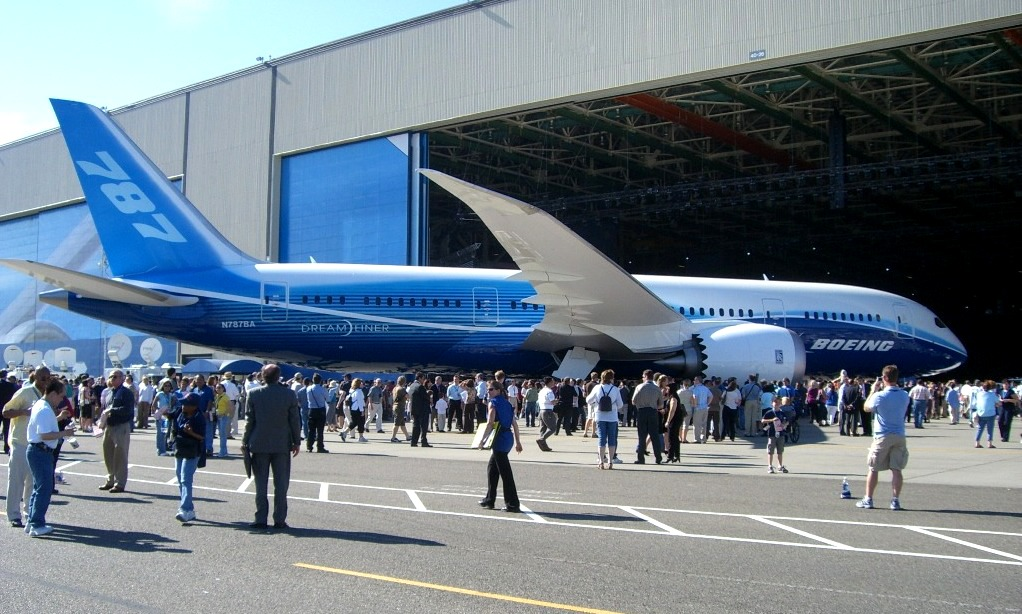
\includegraphics[width=\paperwidth]{dreamliner}};
    \uncover<2->{\node [below right=1cm of dreamliner.north west, anchor=north west]
      {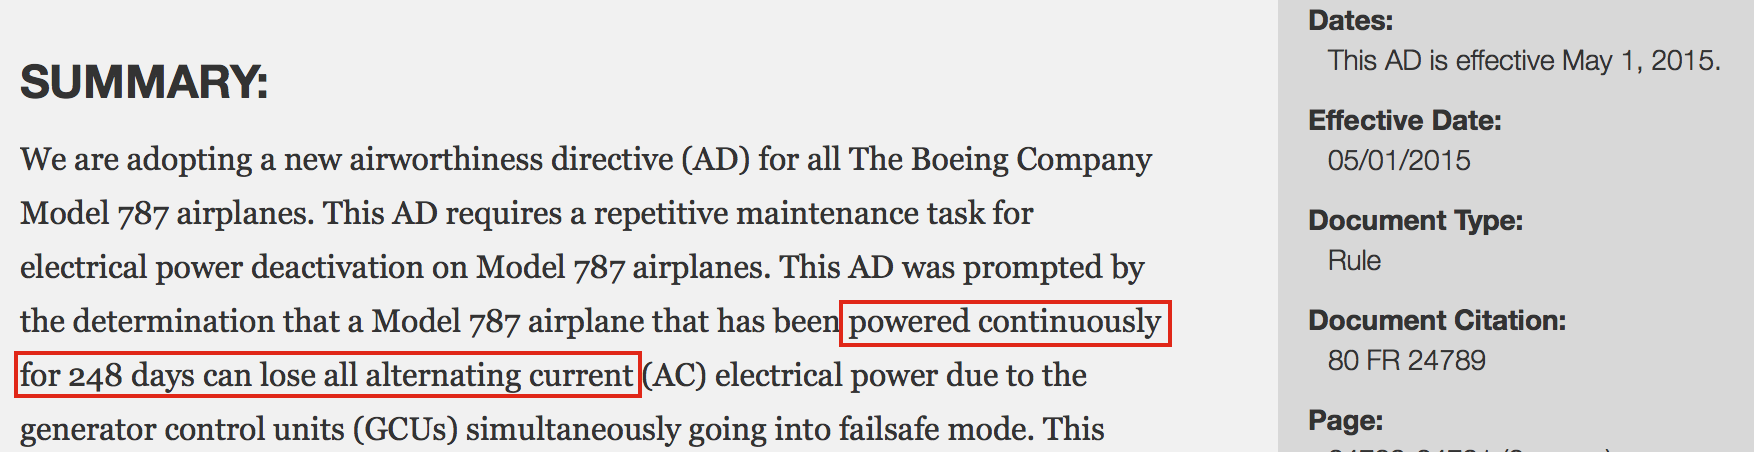
\includegraphics[width=1\framewidth]{dreamliner-bug-2015}};}
    \uncover<3->{\node [above left=1cm of dreamliner.south east, anchor=south east]
      {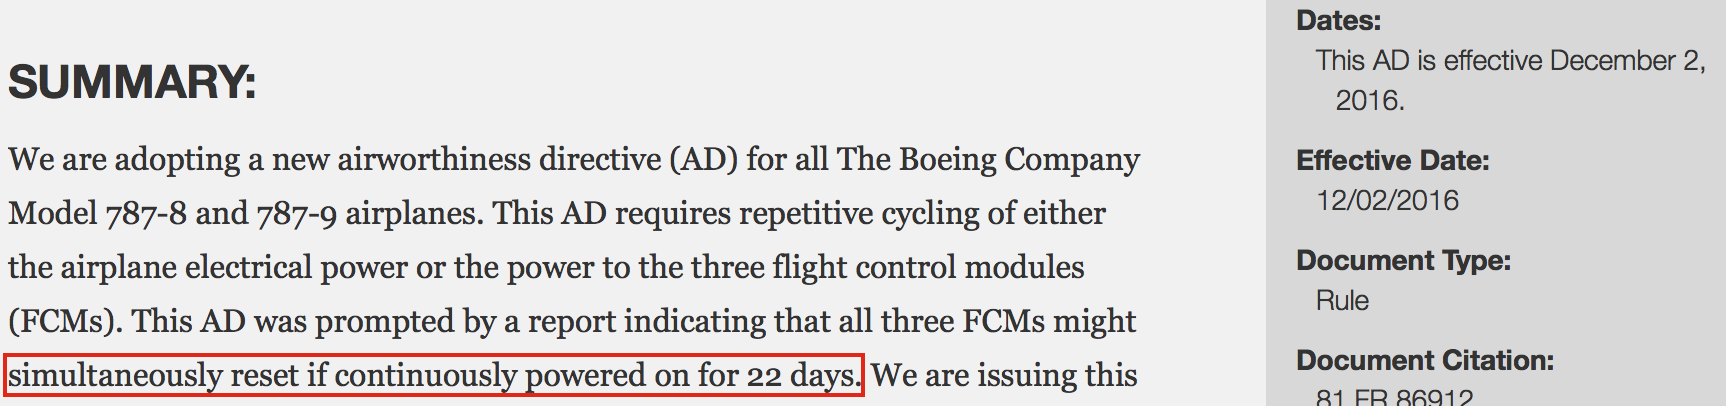
\includegraphics[width=1\framewidth]{dreamliner-bug-2016}};}
  \end{tikzpicture}
\end{frame}

\begin{frame}[fragile]
  \frametitle{The pernicious \texttt{int}}
  Integers are represented either \emph{signed} or \emph{unsigned}
  using a fixed number of \emph{bits}.

  Let's try computing $127+1$, represented as 8bit signed integers.

  \begin{uncoverenv}<2>
  \begin{tikzpicture}
    \matrix (m) [matrix of nodes,
    nodes={minimum size=0.75cm, draw, anchor=center},
    column sep=0pt,
    ]
    { $-2^7$ & $2^6$ & $2^5$ & $2^4$ & $2^3$ & $2^2$ & $2^1$ & $2^0$
      \\};
    \matrix (mfull) [matrix of nodes, below=0.2cm of m,
    nodes={minimum size=0.75cm, draw, anchor=center},
    column sep=0pt,
    ]
    { $0$ & $1$ & $1$ & $1$ & $1$ & $1$ & $1$ & $1$
      \\};
    \node [left=0.1cm of mfull]  {$127$};
    \matrix (mone) [matrix of nodes, below=0.2cm of mfull,
    nodes={minimum size=0.75cm, draw, anchor=center},
    column sep=0pt,
    ]
    { $0$ & $0$ & $0$ & $0$ & $0$ & $0$ & $0$ & $1$
      \\};
    \node [left=0.1cm of mone] {$1$};
    \node [above left=0.1cm and 0.3cm of mone.north west, anchor=center] {$+$};

    \matrix (moops) [matrix of nodes, below=0.2cm of mone,
    nodes={minimum size=0.75cm, draw, anchor=center},
    column sep=0pt,
    ]
    { $1$ & $0$ & $0$ & $0$ & $0$ & $0$ & $0$ & $0$
      \\};
    \node [left=0.1cm of moops] {$-128$};
    \node [above left=0.1cm and 0.3cm of moops.north west, anchor=center] {$=$};
  \end{tikzpicture}
  \end{uncoverenv}
\end{frame}

\begin{frame}[fragile]
  \frametitle{The pernicious \texttt{int}}
  Let's go back and look at the Dreamliner numbers again.

  \begin{equation*}
    248\,\text{days} = 248 \times 24 \times 3600 \times 100 =
    2142720000 \,\text{centiseconds}
  \end{equation*}
  \begin{equation*}
    22\,\text{days} = 22 \times 24 \times 3600 \times 1000 =
    1900800000 \,\text{milliseconds}
  \end{equation*}


  \begin{uncoverenv}<2>
    \begin{equation*}
      \log_2{2142720000} \approx 30.997
    \end{equation*}
  \begin{equation*}
    \log_2{1900800000} \approx 30.824
  \end{equation*}

  Both of these failures are almost certainly due to \emph{integer
    overflow} of a signed 32bit integer.
\end{uncoverenv}
\end{frame}

\begin{frame}[plain,t]
  \begin{flushright}
    \tiny \url{https://cve.mitre.org/cgi-bin/cvekey.cgi?keyword=integer+overflow}
  \end{flushright}
  \begin{tikzpicture}[remember picture, overlay]
    \node[at=(current page.center)]
    {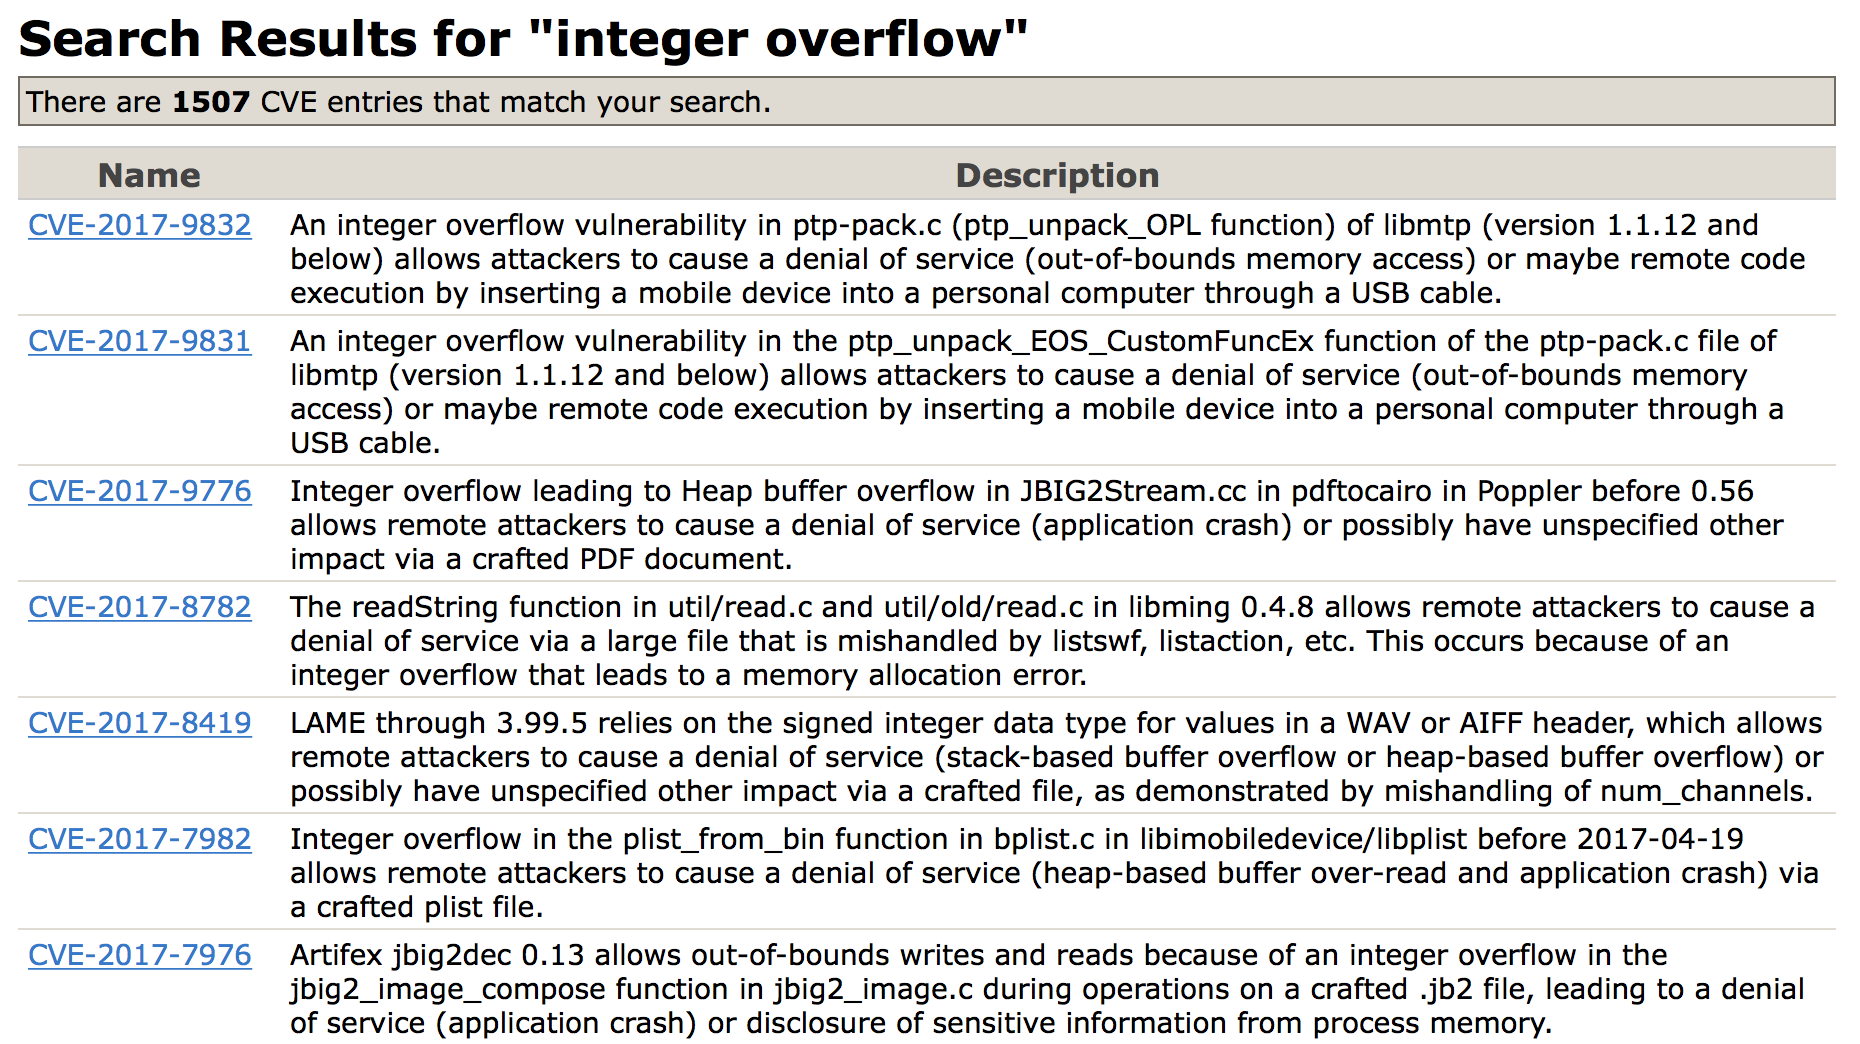
\includegraphics[width=\paperwidth]{cve-overflow}};
  \end{tikzpicture}
\end{frame}

\begin{frame}
  \frametitle{Should you trust your calculation?}

  Computing with real values provides a whole new class of ways to get
  the wrong answer.

  \begin{center}
    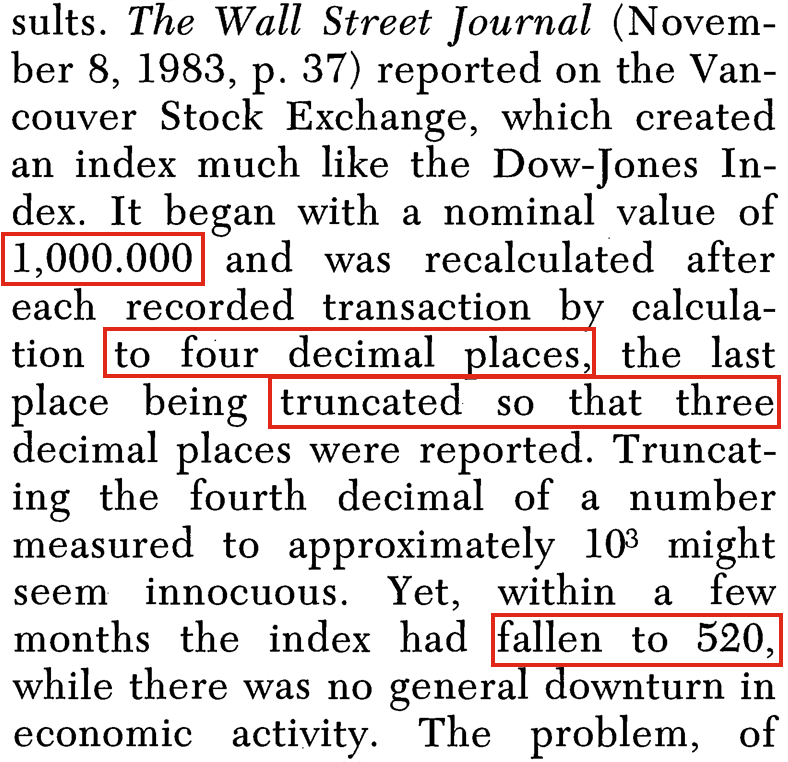
\includegraphics[height=0.6\textheight]{vancouver-index}
  \end{center}
  \begin{flushright}
    {\scriptsize McCullogh \& Vinod, Journal of Economic Literature
    37(2):633--665 (1999)}
  \end{flushright}
\end{frame}

\begin{frame}
  \frametitle{Floating point}
  \begin{itemize}
  \item The real numbers are infinite and uncountable, which presents
    problems on a computer.
  \item We typically approximate real numbers using \emph{floating
      point} numbers.
  \item These take a fixed number of bits (64 for \emph{double
      precision}, 32 for \emph{single}) and split between a
    \emph{significand} and \emph{exponent}, with implicit \emph{base}.
  \end{itemize}
  \begin{equation*}
    1015323 = \underbrace{1.015323}_{\text{significand}} \times \underbrace{10}_{\text{base}}\!\!\!\!\!\!^{\overbrace{6}^{\text{exponent}}}
  \end{equation*}
\end{frame}
\begin{frame}
  \frametitle{Floating point}
  \begin{itemize}
  \item Behaviour implemented in CPUs standardised in IEEE 754
  \item Specifies how to interpret bit patterns as floating point
    numbers
  \item Also specifies \emph{rounding} for calculations that result in
    values not exactly representable
  \end{itemize}
  \begin{tabular}{c|ccc|c}
    Precision & Sign & Exponent & Significand & Total bits \\
    \hline
    single    & 1    & 8        & 23          & 32         \\
    double    & 1    & 11       & 52          & 64         \\
  \end{tabular}
  \begin{tabular}{c|c}
    Precision & Range                                                   \\
    \hline
    single    & {\small $[-3.4028235 \times 10^{38}, 3.4028235 \times 10^{38}]$} \\
    double    & {\small $[-1.7976931348623157\times 10^{308}, 1.7976931348623157 \times 10^{308}]$}
  \end{tabular}
\end{frame}

\begin{frame}
  \frametitle{Addition}
  \begin{itemize}
  \item How to add two numbers with different scales?
    \begin{equation*}
      1 \times 10^{6} + 2
    \end{equation*}
  \item \emph{Normalise} representation (so exponent is the same)
  \item add significands
    \begin{align*}
      1 \times 10^{6} + 2 &= \\
      1 \times 10^{6} + 0.000002 \times 10^{6} &= \\
      1.000002 \times 10^{6}
    \end{align*}
  \item What happens if there are not enough bits in the significand?
  \end{itemize}
\end{frame}

\begin{frame}[fragile]
  \frametitle{No associativity}
  We expect that arithmetic operations \emph{associate}
  \begin{equation*}
    (a + b) - c = a + (b - c).
  \end{equation*}

  Floating point operations do not.

  \begin{center}
    \begin{onlyenv}<2>
\begin{minted}[fontsize=\small]{c}
float a = 1f;
float b = 1e10f;
print ((a + b) - b);
print (a + (b - b));
\end{minted}
    \end{onlyenv}
  \end{center}
  \begin{center}
    \begin{onlyenv}<3>
\begin{minted}[fontsize=\small]{c}
float a = 1f;
float b = 1e10f;
print ((a + b) - b); => 0.0
print (a + (b - b)); => 1.0
\end{minted}
    \end{onlyenv}
  \end{center}
\end{frame}

\begin{frame}[fragile]
  \frametitle{Just add more precision, no?}

  \begin{itemize}
  \item a \emph{single precision} \texttt{float} has about 8 decimal
    digits of precision.
  \item So $1\times10^{10} + 1 = 1\times10^{10} + 0.000,000,000,1\times10^{10} = 1$.
  \item We could have used a \emph{double precision} \texttt{double}
    instead (16 decimal digits).
  \item In this case we have enough digits so we end up with
    $1.000,000,000,1\times10^{10}$.
  \item Which suggests we should always calculate in double precision
    for ``more accuracy''.
  \end{itemize}

  \begin{uncoverenv}<2->
    \begin{columns}
      \begin{column}{0.5\textwidth}
        \begin{onlyenv}<2>
\begin{minted}[fontsize=\scriptsize]{c}
int count = 0;
float x = 0;
for (x=0; x<1.0f; x+=1.0f/6.0f)
    count += 1
printf("%d\n", count)
\end{minted}
        \end{onlyenv}
        \begin{onlyenv}<3->
\begin{minted}[fontsize=\scriptsize]{c}
int count = 0;
float x = 0;
for (x=0; x<1.0f; x+=1.0f/6.0f)
    count += 1
printf("%d\n", count) => 6
\end{minted}
        \end{onlyenv}
      \end{column}
      \begin{column}{0.5\textwidth}
        \begin{onlyenv}<2-3>
\begin{minted}[fontsize=\scriptsize]{c}
int count = 0;
double x = 0;
for (x=0; x<1.0; x+=1.0/6.0)
    count += 1
printf("%d\n", count)
\end{minted}
        \end{onlyenv}
        \begin{onlyenv}<4->
\begin{minted}[fontsize=\scriptsize]{c}
int count = 0;
double x = 0;
for (x=0; x<1.0; x+=1.0/6.0)
    count += 1
printf("%d\n", count) => 7
\end{minted}
        \end{onlyenv}
      \end{column}
    \end{columns}
  \end{uncoverenv}
\end{frame}
\end{document}
